
% ??ds define the errors properly Refer to ODE LLG section.
% ??ds same y-axis on ml error plots?
% ??ds add a table of # renormalisations?

% ??ds what's up with that initial transient in the ml err of sc-llg?

\FloatBarrier
\chapter{Alternative magnetisation re-normalisation methods}
\label{sec:magn-renorm-meth}
\chaptermark{Alternative re-normalisation}

In this \thisref{sec:magn-renorm-meth} we experimentally compare three methods for re-normalising the magnetisation:
\begin{enumerate}
\item Re-normalisation after every step, the simplest magnetisation re-normalisation method.
\item The self-correcting LLG method used by \nmag (described in \cref{sec:sc-llg}).
\item Tolerance-based re-normalisation used by \magpar (described in \cref{sec:ensuring-constant-mv}).
\end{enumerate}

As our example problem we use the relaxing nano-sphere described in \cref{sec:imr-ode-llg-numer-exper}.

\section{Implementation details}

As in \cref{sec:impl-deta-ode-llg} we use the Landau-Lifshitz (LL) form of the LLG.
The Newton-Raphson method is used for linearisation with the Jacobian calculated analytically and solved using a direct solver.
The Newton-Raphson tolerance set to $\ntol = 10^{-8}$.
We use BDF2 for these experiments because we need a time integrator with no geometric integration properties in order to properly test the re-normalisation methods (TR is equivalent to IMR for the undamped ODE LLG problem so it has the same geometric integration properties in this case, see \cref{sec:aimr-llgode-numerical-results}).
The time step size is fixed at $\dtn = 0.1$.

Tolerance-based re-normalisation is implemented as follows:
if the error in the magnetisation length, $\errml = \abs{1 - \abs{\mv}}$, is less than the tolerance, $\mltol$, then nothing is done and the integration continues.
On the other hand if $\errml > \mltol$ then we set $\mv_{i}$ to $\mv_{i}/\abs{\mv_{i}}$ for the values of the magnetisation at all times stored by the time integrator (for BDF2 this corresponds to $i=n+1, n, n-1$).
Note that re-normalising the history values of TR is more complex because one of them is a derivative (at least in our implementation, see \cref{eq:impl-tr}), which would need to be recalculated using the newly re-normalised magnetisation values for consistency.

We use tolerance values of $\mltol = 0, 10^{-6}, 10^{-2}, 10^{200}$.
Note that $\mltol \gg 1$ (\eg $\mltol = 10^{200}$) corresponds to no re-normalisation, while $\mltol = 0$ corresponds to re-normalisation after every time step.
The default value used in \magpar\footnote{Based on the source code of version 0.9, the relevant function is \texttt{CheckIterationLL\_Init}.} is $\mltol = 10^{-2}$.

The self correcting LLG is implemented by replacing the standard residual, $\rv_{\mathrm{ll}}$ given in \cref{eq:r-ode-llg}, with the modified residual
\begin{equation}
  \rv = \rv_{\mathrm{ll}}  - \scc \mv \bigb{1 - \abs{\mv}^2},
\end{equation}
where $\scc$ is a parameter that can be tuned.
The Jacobian of the modified residual is given by
\begin{equation}
  \label{eq:J-ode-sc-llg}
  \Jm = \Jm_{\mathrm{ll}} + 2\scc \bigb{\mv \tensorprod \mv} - \scc \bigb{1 - \abs{\mv}^2} \Idm ,
\end{equation}
where $\Jm_{\mathrm{ll}}$ is the Jacobian of $\rv_{\mathrm{ll}}$ and is given in \cref{eq:J-ode-llg}.

We experiment with a range of parameter values: $\scc = 0, 0.1, 1, 10, 100, 1000$.
Larger values were not used because the Newton-Raphson method often failed to converge within ten steps for $\scc \gtrsim 1000$.

Note that, due to implementation details, values are output \emph{after} any re-normalisation for that step has been performed.


\section{Results: tolerance-based renormalisation}
\label{sec:renorm-after-toler}

\begin{figure}
  \centering
  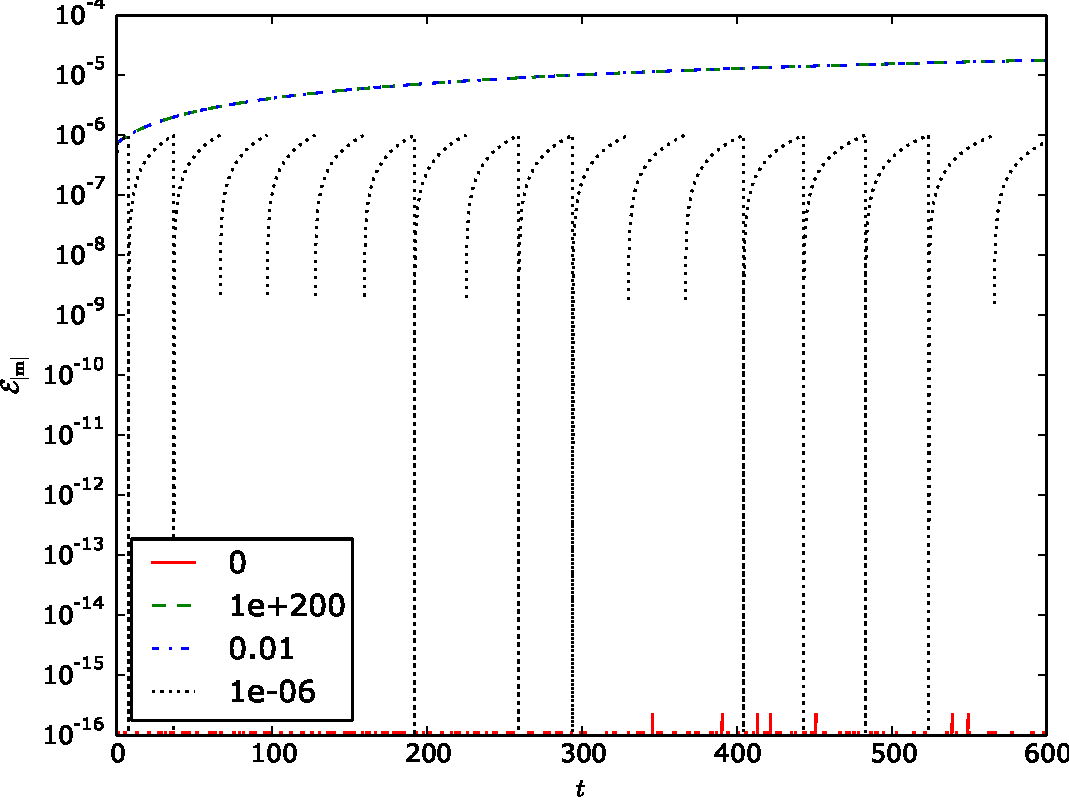
\includegraphics[width=0.8\textwidth]{{{plots//tolrenorm-geom-properties/0-mlengtherrormaxesvstimes}}}
  \caption{
    Error in magnetisation length, $\errml$, over time
    for the relaxing nano-sphere problem with
    $\dampc = 0$.
    Magnetisation length is enforced by tolerance-based renormalisation,
    the legend indicates the value of the tolerance $\mltol$.
  }
  \label{fig:renorm-tol-ml-err-undamped}
\end{figure}

\begin{figure}
  \centering
  \includegraphics[width=0.8\textwidth]{{{plots/tolrenorm-geom-properties/0.01-mlengtherrormaxesvstimes}}}
  \caption{
    Error in magnetisation length, $\errml$, over time
    for the relaxing nano-sphere problem
    with $\dampc = 0.01$.
    Magnetisation length is enforced by tolerance-based renormalisation,
    the legend indicates the value of the tolerance $\mltol$.
  }
  \label{fig:renorm-tol-ml-err}
\end{figure}

In \cref{fig:renorm-tol-ml-err-undamped,fig:renorm-tol-ml-err} we show the error in the magnetisation length over time
\begin{equation}
  \errml = \abs{\abs{\mv} - 1}
\end{equation}
for various values of $\mltol$ and $\dampc=0.01, 0$ respectively.
For the case with $\dampc = 0.01$ and $\mltol = 10^{-6}$ re-normalisation is performed with increasing frequency until $t \gtrsim 280$, after which it is performed after almost every step.
In both the damped and undamped cases, the use of the intermediate tolerance value, $\mltol = 10^{-6}$, results in oscillations of the magnetisation length.
For $\mltol = 10^{-2}$ in the undamped case the error in the magnetisation length never reaches the tolerance and the behaviour is identical to the case of no re-normalisation.
In the damped case the tolerance $\mltol = 10^{-2}$ is reached and the behaviour is similar to that of $\mltol = 10^{-6}$, except that the oscillations in the magnetisation length begin at a later time.


\begin{figure}
  \centering
  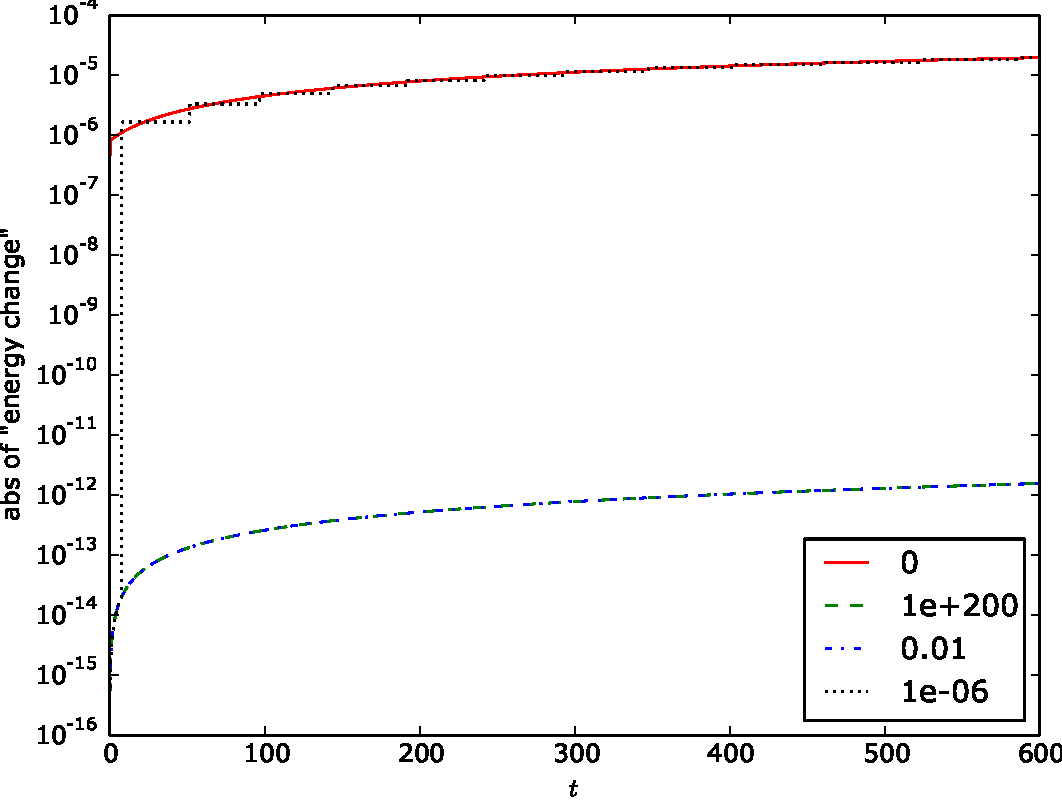
\includegraphics[width=0.8\textwidth]{plots/tolrenorm-geom-properties/0-absofenergychangevstimes.pdf}
  \caption{
    Error in energy over time
    for the relaxing nano-sphere problem
    with $\dampc = 0$.
    Magnetisation length is enforced by tolerance-based renormalisation,
    the legend indicates the value of the tolerance $\mltol$.
  }
  \label{fig:renorm-tol-energy-err}
\end{figure}

In \cref{fig:renorm-tol-energy-err} the errors in the energy for the undamped case are shown.
As noted previously, $\mltol= 10^{-2}$ behaves as the non-renormalised case for this example.
When $\mltol = 10^{-6}$ we see an error similar to that for the always re-normalised case, except with additional oscillations in the energy corresponding to times where a re-normalisation is carried out.


\begin{figure}
  \centering
  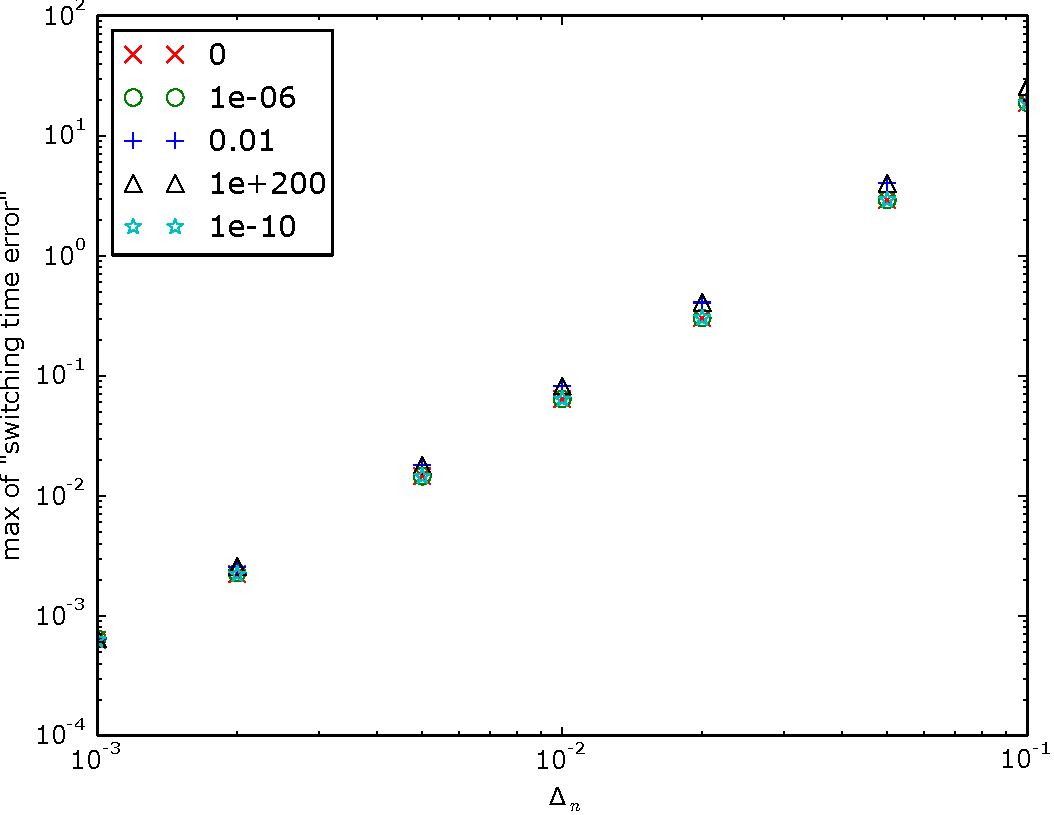
\includegraphics[width=0.8\textwidth]{plots/tolrenorm_llg_ode_convergence/maxofswitchingtimeerrorvsmeanofdts}
  \caption{
    Convergence of the maximum (over all steps) of the error in the switching time
    against step size
    for the relaxing nano-sphere problem with
    $\dampc = 0.01$.
    Magnetisation length is enforced by tolerance-based renormalisation,
    the legend indicates the value of the tolerance $\mltol$.
    ??ds not actually a mean...
  }
  \label{fig:tol-renorm-convergence}
\end{figure}

Finally in \cref{fig:tol-renorm-convergence} we show the convergence of the method (in terms of the error in the switching time) as the step size is reduced for the damped case.
The use of $\mltol=10^{-2}$ or no re-normalisation ($\mltol=10^{200}$) gives slightly worse errors than the tighter tolerances.


\FloatBarrier
\section{Results: the self-correcting LLG}
\label{sec:self-correcting-llg-results}

\begin{figure}
  \centering
  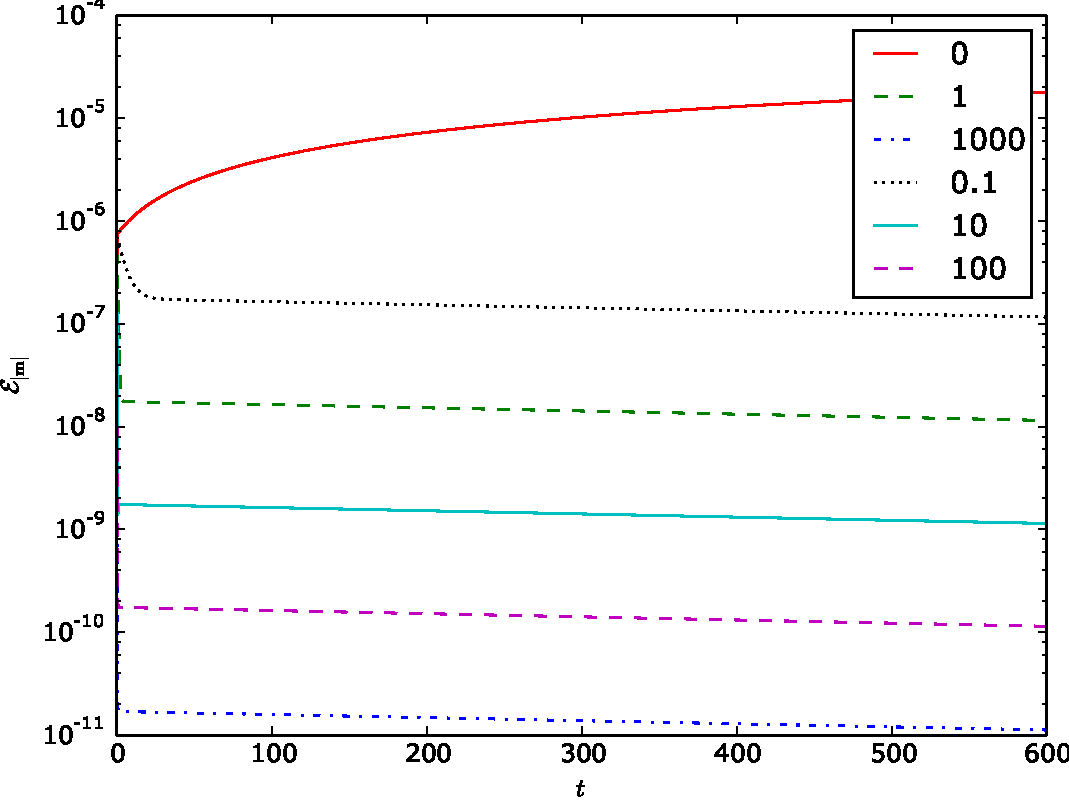
\includegraphics[width=0.8\textwidth]{plots/sc-geom-properties/0-mlengtherrormaxesvstimes.pdf}
  \caption{
    Error in magnetisation length, $\errml$, over time
    for the relaxing nano-sphere problem
    with $\dampc = 0$.
    Magnetisation length is enforced by use of the self-correcting LLG.
   The legend indicates the values of $\scc$.
  }
  \label{fig:sc-ml-err-undamped}
\end{figure}

\begin{figure}
  \centering
  \includegraphics[width=0.8\textwidth]{{{plots/sc-geom-properties/0.01-mlengtherrormaxesvstimes}}}
  \caption{
    Error in magnetisation length, $\errml$, over time
    for the relaxing nano-sphere problem
    with $\dampc = 0.01$.
    Magnetisation length is enforced by use of the self-correcting LLG,
    the legend indicates the values of $\scc$.
  }
  \label{fig:sc-ml-err}
\end{figure}


In \cref{fig:sc-ml-err-undamped,fig:sc-ml-err} we show the errors in magnetisation length over time with various values of the parameter $\scc$ for the damped and undamped problems respectively.
As would be expected larger values of $\scc$ reduce the error in both cases.
Note that in the damped case (\cref{fig:sc-ml-err}) with $\scc = 1000$ the curve stops at $t \sim 480$, this is due to non-convergence of the Newton-Raphson method within the ten iteration limit.

\begin{figure}
  \centering
  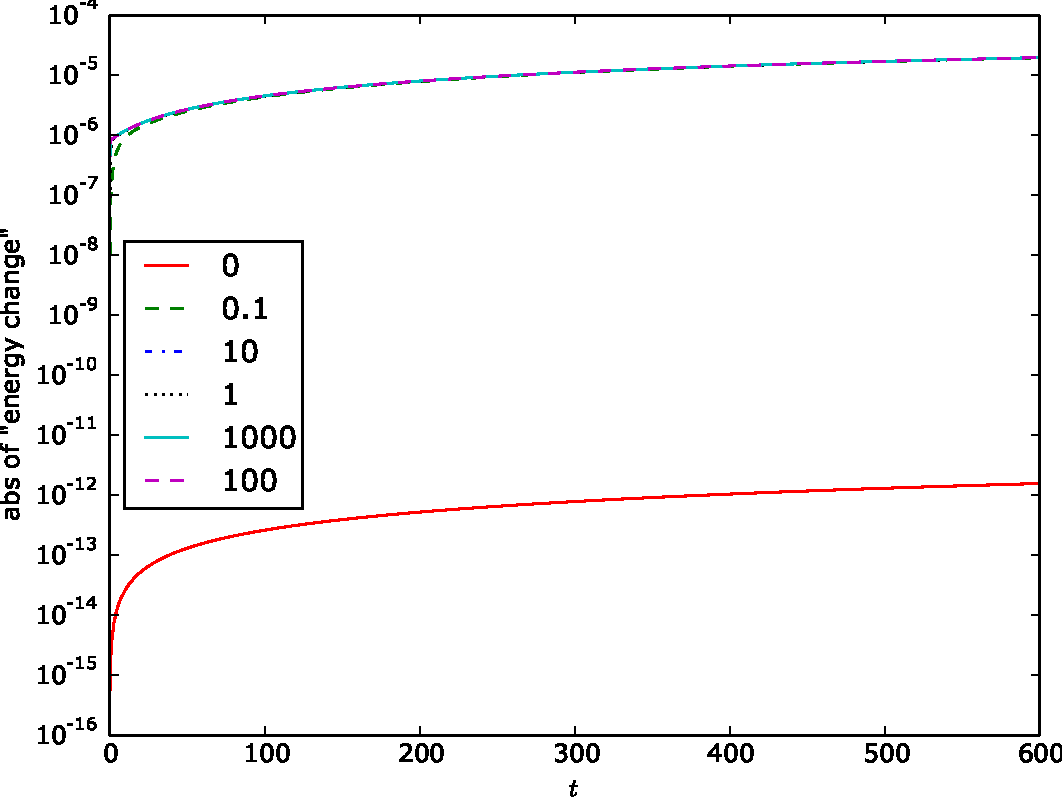
\includegraphics[width=0.8\textwidth]
  {{{plots/sc-geom-properties/0-absofenergychangevstimes}}}
  \caption{
    Error in energy over time
    for the relaxing nano-sphere problem
    with $\dampc = 0$.
    Magnetisation length is enforced by use of the self-correcting LLG,
    the legend indicates the values of $\scc$.
  }
  \label{fig:sc-energy-err}
\end{figure}

In \cref{fig:sc-energy-err} we show the error in the energy for the undamped problem for various values of the parameter $\scc$.
We see that any $\scc > 0$ causes an error in the energy similar to that caused by the various re-normalisation approaches shown in \cref{fig:renorm-tol-energy-err}.


\begin{figure}
  \centering
  \includegraphics[width=0.8\textwidth]
  {{{plots/self_correcting_llg_ode_convergence/maxofswitchingtimeerrorvsmeanofdts}}}
  \caption{
    Convergence of the maximum (over all steps) of the error in the switching time
    against step size
    for the relaxing nano-sphere problem with
    $\dampc = 0.01$.
    Magnetisation length is enforced by use of the self-correcting LLG or re-normalisation after every step (\ie tolerance based renormalisation with $\mltol = 0$).
    The legend indicates, respectively, the values of $\scc$ and the tolerance $\mltol$.
  }
  \label{fig:sc-convergence}
\end{figure}

In \cref{fig:sc-convergence} we show the convergence of the maximum error in the switching time against the time step size $\dtn$ with two values of $\scc$.
For comparison we also show the results when re-normalisation after every step is used instead of the self correcting term (\ie $\mltol = 0$ and $\scc = 0$).
We see that the resulting errors are essentially identical for all three cases.

\begin{table}
  \begin{subtable}{.5\textwidth}
    \centering
    \begin{tabular}{ll}
      $\scc$ & Mean Newton iterations \\
      \hline
      0 & 2.0 \\
      0.1 & 2.0 \\
      1 & 2.46 \\
      10 & 2.68 \\
      100 & 3.13 \\
      1000 & 3.12* \\
    \end{tabular}%
    \caption{Solved with BDF2 and $\ntol = 10^{-8}$. Magnetisation length is enforced by use of the self-correcting LLG.}
  \end{subtable}%
  \begin{subtable}{.5\textwidth}
    \centering
    \begin{tabular}{ll}
      $\scc$ & Mean Newton iterations \\
      \hline
      0 & 2.0 \\
      0.1 & - \\
      1 & - \\
      10 & - \\
      100 & - \\
      1000 & - \\
    \end{tabular}%
    \vfill
    \caption{Solved with IMR and $\ntol = 10^{-12}$}
  \end{subtable}%
  \caption{
    Mean number of Newton iterations (over all time steps) for convergence
    for the relaxing nano-sphere problem with
    $\dampc = 0.01$.
    The time integration methods used are indicated in the sub-captions.
    Values of $\scc \neq 0$ are not considered when using IMR because no self-correcting term is needed to conserve $\abs{\mv}$.
    Note that with $\scc = 1000$ the Newton-Raphson method fails to converge at $t \sim 480$.
  }
  \label{tab:sc-newton-iters}
\end{table}


In \cref{tab:sc-newton-iters} we show the number of Newton-Raphson iterations required for convergence for each value of $\scc$.
For comparison we also show the result when using IMR with Newton tolerance $\ntol=10^{-12}$ (recall that a sharp linearisation tolerance is required for IMR to attain good geometric integration properties).
We see that as $\scc$ is increased the mean number of Newton iterations to converge also increases.
In addition we see that the tighter tolerance required for geometric integration with IMR has no effect on the number of iterations required.

Since $\scc \geq 100$ is required to control $\errml$ to even the fairly loose tolerance of $10^{-6}$, the use of the self correcting LLG requires, on average, at least one additional Newton-Raphson iteration per time step.
As the majority of the computation time for a time step is spent within the Newton-Raphson method, this increases the cost of each step by approximately $50\%$.
Since the use of the self correcting LLG does not provide any improvement in the overall accuracy or energy error over re-normalising after every step (so the same $\dtn$ is required to obtain the same accuracy), this increases the overall cost of the method by the same factor.

\begin{figure}
  \centering
  \includegraphics[width=\textwidth]{{{plots/sc-adaptivity/maxofswitchingtimeerrorvsmeanofdts}}}
  \caption{
    Convergence of the maximum (over all steps) of the error in the switching time
    against step size
    for the relaxing nano-sphere problem with
    $\dampc = 0.01$
    solved using adaptive BDF2.
    Magnetisation length is enforced by use of the self-correcting LLG or re-normalisation after every step (\ie tolerance based renormalisation with $\mltol = 0$).
    The legend indicates, respectively, the values of $\scc$ and the tolerance $\mltol$.
  }
  \label{fig:sc-adaptivity-convergence}
\end{figure}

Finally we study the effect of the use of the self-correcting LLG on adaptive time integration.
Since the self correcting term is part of the differential equation (as opposed to standard renormalisation, which is carried out separately) we might expect adaptive time integration methods to be able to better predict the error, and choose more appropriate step sizes.
In \cref{fig:sc-adaptivity-convergence} we show the convergence behaviour when using adaptive BDF2 (as described in \cref{sec:aimr-implementation}) with tolerances of $\toltt = 10^{-4}, 3\E{-5}, 10^{-5}, 3\E{-6}, 10^{-6}, 3\E{-7}, 10^{-7}, 10^{-8}$ with various values of $\scc$.
For comparison we also show the convergence behaviour when the magnetisation is re-normalised after every step.
If the use of the self-correcting LLG is beneficial we would expect to see lower errors for the same average step size, but the plots are indistinguishable.


\section{Conclusions}

By design, the use of tolerance-based renormalisation allows larger errors to appear in $\abs{\mv}$ than re-normalisation after every step.
It also introduces spurious oscillations in $\abs{\mv}$ and in the error in the energy for the undamped case.
It has a slight negative effect on convergence when compared to re-normalisation after every step, and no effect on the computational cost of the re-normalisation.

The self correcting LLG is worse at controlling errors in $\abs{\mv}$ than re-normalisation after each step, and gives very similar errors in the energy.
It gives essentially identical convergence properties as re-normalisation after every step.
Finally, it requires additional step(s) of the Newton-Raphson method convergence (typically one more step is needed, increasing the computation time for the simulation by a factor of $\sim 50\%$).

Hence there appears to be no obvious reason to prefer either tolerance-based renormalisation or the self correcting LLG over re-normalisation after every step for ODE problems.
Since the methods used here match those used for PDE problems, except for the obvious lack of any spatial discretisation, this conclusion is likely to extend to PDE problems.


%%% Local Variables:
%%% mode: latex
%%% TeX-master: "main"
%%% End:
